\documentclass[dvipdfmx]{jarticle}
\hoffset=-25mm
\voffset=-20mm
\pagestyle{empty}
\usepackage{graphicx}
\usepackage{color}
\usepackage{latexsym}
\usepackage{amssymb}
\usepackage{wrapfig}
\usepackage{xcolor}
\usepackage{tikz}
\usetikzlibrary{calc,shapes}
\usepackage{fancyvrb}
\usepackage{url}
\newcounter{coffee}
\newcounter{bean}
\newcounter{figcnt}
\newcommand{\tuple}[1]{\langle{#1}\rangle}

\setlength{\textheight}{25.5cm}
\setlength{\textwidth}{17cm}

%\deflinenumfalse % 定義番号を表示しない

\usepackage{amsmath}	% required for `\cases' (yatex added)
\begin{document}
\begin{flushright}
    \verb|2026/11/13|
\end{flushright}
\begin{center}
    {\Large\bf コンパイラ 第７回演習課題}
\end{center}

%{\color{red}提出期限を12/5に延長します．}

\begin{itemize}
    \item TACTの課題の添付ファイルとしてPDFファイルで提出すること．
    \item 手書きレポートをPDFとして提出する方法は講義webサイトを
          参照\footnote{\url{https://sites.google.com/sqlab.jp/26compiler/how-to-make-report}}すること．
    \item 提出期限: {11月20日（金）23:55}
\end{itemize}

\begin{list}{[\arabic{coffee}]}{\usecounter{coffee}}
    \item 以下のプログラムの関数\texttt{sort}は末尾再帰(末端再帰)である．（バブルソートの再帰版）
          再帰呼び出しを消去し,同じ振る舞いをするwhile文(あるいはfor文)のループによるプログラムに変換せよ．

          \begin{minipage}{.7\textwidth}
              \VerbatimInput[frame=single,numbers=left]{bubble-sort.txt}
          \end{minipage}

          ヒント：講義資料と同様に,4行目にラベルL:をつけて7行目の\texttt{sort}の再帰呼び出しをgoto Lに置き換えるとどうなるか？

    \item 図\ref{fig:progssa}に示す3番地コードについて答えよ．
          変数の型はすべて整数型とする．
          \begin{center}
              \begin{tabular}{ccccc}
                  %	 \includegraphics[scale=.85]{figs/prog.epsi} 
                  \scalebox{0.75}{
                      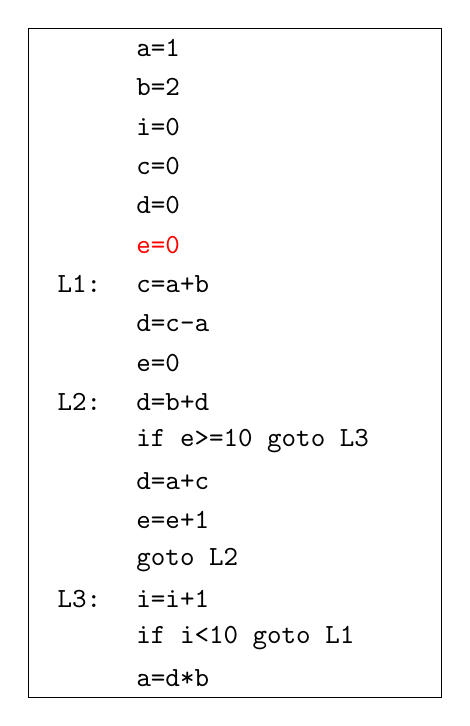
\begin{tikzpicture}
                          \draw[draw] (-0.25,0.25) rectangle (5,-8.25);
                          \node[anchor=west] at (1,0) {\texttt{a=1}};
                          \node[anchor=west] at (1,-0.5) {\texttt{b=2}};
                          \node[anchor=west] at (1,-1) {\texttt{i=0}};
                          \node[anchor=west] at (1,-1.5) {\texttt{c=0}};
                          \node[anchor=west] at (1,-2) {\texttt{d=0}};
                          \node[anchor=west] at (1,-2.5) {\color{red}\texttt{e=0}};
                          \node[anchor=west] at (0,-3) {\texttt{L1:}};
                          \node[anchor=west] at (1,-3) {\texttt{c=a+b}};
                          \node[anchor=west] at (1,-3.5) {\texttt{d=c-a}};
                          \node[anchor=west] at (1,-4) {\texttt{e=0}};
                          \node[anchor=west] at (0,-4.5) {\texttt{L2:}};
                          \node[anchor=west] at (1,-4.5) {\texttt{d=b+d}};
                          \node[anchor=west] at (1,-5) {\texttt{if e>=10 goto L3}};
                          \node[anchor=west] at (1,-5.5) {\texttt{d=a+c}};
                          \node[anchor=west] at (1,-6) {\texttt{e=e+1}};
                          \node[anchor=west] at (1,-6.5) {\texttt{goto L2}};
                          \node[anchor=west] at (0,-7) {\texttt{L3:}};
                          \node[anchor=west] at (1,-7) {\texttt{i=i+1}};
                          \node[anchor=west] at (1,-7.5) {\texttt{if i<10 goto L1}};
                          \node[anchor=west] at (1,-8) {\texttt{a=d*b}};
                      \end{tikzpicture}}
                                        & \qquad &
                  %\includegraphics[scale=.8]{figs/cfg-r1.epsi}
                  \scalebox{0.8}{
                      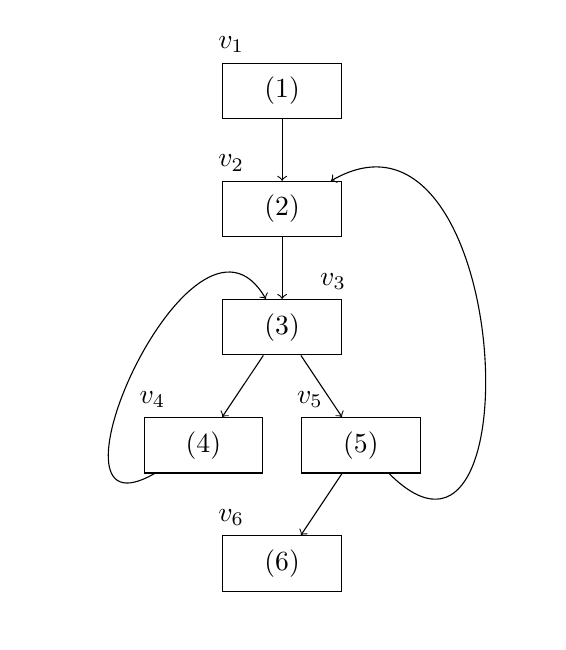
\begin{tikzpicture}%[node distance=2cm]
                          \node [draw,rectangle,label=above left:$v_1$,inner xsep=15pt,inner ysep=5pt]
                          (V1) at (0,0) {(1)};
                          \node [draw,rectangle,label=above left:$v_2$,inner xsep=15pt,inner ysep=5pt]
                          (V2) at ($(V1)+(0,-1.5)$) {(2)};
                          \node [draw,rectangle,label=above right:$v_3$,inner xsep=15pt,inner ysep=5pt]
                          (V3) at ($(V2)+(0,-1.5)$) {(3)};
                          \node [draw,rectangle,label=above left:$v_4$,inner xsep=15pt,inner ysep=5pt]
                          (V4) at ($(V3)+(-1,-1.5)$) {(4)};
                          \node [draw,rectangle,label=above left:$v_5$,inner xsep=15pt,inner ysep=5pt]
                          (V5) at ($(V3)+(1,-1.5)$) {(5)};
                          \node [draw,rectangle,label=above left:$v_6$,inner xsep=15pt,inner ysep=5pt]
                          (V6) at ($(V5)+(-1,-1.5)$) {(6)};
                          \path[->] (V1) edge (V2)
                          (V2) edge (V3)
                          (V3) edge (V4)
                          (V3) edge (V5)
                          (V5) edge (V6);
                          \draw[->] (V5) to [out=315,in=30,looseness=1.8] (V2);
                          \draw[->] (V4) to [out=210,in=120,looseness=1.8] (V3);
                      \end{tikzpicture}}
                                        & \qquad &
                  %	 \includegraphics[scale=.8]{figs/cfg2-r1.epsi}
                  % \scalebox{0.8}{
                  % 	\begin{tikzpicture}%[node distance=2cm]
                  % 	 \node [draw,rectangle,label=above left:$v_1$,inner xsep=15pt,inner ysep=5pt] 
                  % 	 (V1) at (0,0) {(B1)};
                  % 	 \node [draw,rectangle,label=above left:$v_2$,inner xsep=15pt,inner ysep=5pt] 
                  % 	 (V2) at ($(V1)+(0,-1.5)$) {
                  % 		 (B2)
                  % 		 };
                  % 	 \node [draw,rectangle,label=above right:$v_3$,inner xsep=15pt,inner ysep=5pt] 
                  % 	 (V3) at ($(V2)+(0,-1.5)$) {(3)};
                  % 	 \node [draw,rectangle,label=above left:$v_4$,inner xsep=15pt,inner ysep=5pt] 
                  % 	 (V4) at ($(V3)+(-1,-1.5)$) {(4)};
                  % 	 \node [draw,rectangle,label=above left:$v_5$,inner xsep=15pt,inner ysep=5pt] 
                  % 	 (V5) at ($(V3)+(1,-1.5)$) {(5)};
                  % 	 \node [draw,rectangle,label=above left:$v_6$,inner xsep=15pt,inner ysep=5pt] 
                  % 	 (V6) at ($(V5)+(-1,-1.5)$) {(6)};
                  % 	 \path[->] (V1) edge (V2)
                  % 						 (V2) edge (V3)
                  % 						 (V3) edge (V4)
                  % 						 (V3) edge (V5)
                  % 						 (V5) edge (V6);
                  % 	 \draw[->] (V5) to [out=315,in=30,looseness=1.8] (V2);
                  % 	 \draw[->] (V4) to [out=210,in=120,looseness=1.8] (V3);
                  % 	\end{tikzpicture}}
                  \\
                  \refstepcounter{figcnt}図\thefigcnt
                  \label{fig:progssa}   &        &
                  \refstepcounter{figcnt}
                  図\thefigcnt
                  \label{fig:flowgraph} &        &
                  %  \refstepcounter{figcnt}
                  %    		 図\thefigcnt
                  %  \label{fig:flowgraphtwo}
              \end{tabular}
          \end{center}
          \begin{list}%
              {(\arabic{bean})} %default label
              {\usecounter{bean}} %formatting parameter
              \item フローグラフを構成すると図\ref{fig:flowgraph}のようになる．それぞれのノードに
                    含まれる3番地コードを答えよ．
              \item このフローグラフに対する支配木を示せ．
              \item 図\ref{fig:flowgraph}の各頂点に対する支配辺境$DF$を計算せよ．
                    $\mathtt{a}$, $\mathtt{b}$, $\mathtt{c}$, $\mathtt{d}$の各
                    変数に対して$\phi$関数を挿入すべきノードの集合
                    $DF^+(S^a_0)$, $DF^+(S^b_0)$, $DF^+(S^c_0)$, $DF^+(S^d_0) $
                    を求めよ．(ここで，$S^a_0$，$S^b_0$， $S^c_0$, $S^d_0$は，
                    それぞれ変数$\mathtt{a}$, $\mathtt{b}$, $\mathtt{c}$,
                    $\mathtt{d}$が定義されているノードの集合を表す．
              \item フローグラフの節点に3番地コードを書きこんだグラフに
                    $\phi$関数を挿入し，添え字を決定してSSA形式に変換したフロー
                    グラフ図を示せ．
                    % \item 前問で得られるフローグラフに機械的にノードを加えることで
                    %       $\phi$関数を除去したフローグラフを示せ．
                    %       %  \item 前問で追加したノードで計算に必要なノードはどれか．
                    % \item 結果的に変数$b$は不要で最適化で消去できる．その方法と理由
                    %       を説明せよ．
          \end{list}
\end{list}
\end{document}
